\documentclass[pdf,rico,slideColor,colorBG]{prosper}

\usepackage{amsmath}
\usepackage{graphics}
\begin{document}

%% ------------------------------------------------------------
\begin{slide}{The Library Infrastructure Project}
\begin{center}Isaac Jones

HIM: Saturday 29 August, 2003\end{center}
\end{slide}

%% ------------------------------------------------------------
\begin{slide}{Our Thanks to $\lambda \mu$}
\begin{itemize}
\item For the use of his lazer pointer
\item Lambda's Namesake:
\item 
\includegraphics{stoneCat.eps}  
\includegraphics[width=.4\textwidth]{cartoonCat.eps} 
\includegraphics[width=.2\textwidth]{lambda.eps}
\end{itemize}
\end{slide}

%% ------------------------------------------------------------
%% \begin{slide}{Terminology}

%% \end{slide}


%% ------------------------------------------------------------
%% Introduction Section
%% ------------------------------------------------------------

%% ------------------------------------------------------------
\begin{slide}{Overview \& Goals}
%% What is this project and why is it needed
\begin{itemize}
  \item ``Languages flourish when libraries are plentiful, reliable, and well documented.'' -- SPJ
  \item Currently, there is no great way for tool authors to contribute and widely distribute their libraries and tools
  \item Except to have them included with the implementations.
  \item BUT... This is a strain on the implementation \& library authors.
  \item Lets give library \& tool authors a way to ``contribute'' their software
\end{itemize}
\end{slide}

%% ------------------------------------------------------------
\begin{slide}{Issues Facing 3rd Party Tool Authors}
\begin{itemize}
  \item Difficult to distribute binary Haskell libraries
  \item ... so the end user must build (and rebuild) all the libraries on their own system
  \item ... but there is no standard build system
  \item ... all of which make it hard to build Debian packages (for instance)
\end{itemize}
\end{slide}

% Slide about Numeric-Quest code?

%% ------------------------------------------------------------
\begin{slide}{...Issues Facing 3rd Party Tool Authors}
\begin{itemize}
  \item Several Haskell implementations which treat ``packages'' differently (different binary formats, different means of collecting packages)
  \item Language extensions and supporting libraries are a moving target (and oh, so tempting), causing the bitrot of tools that aren't actively maintained
  \item No way to express dependency on particular libraries, compilers, or versions thereof (job of the packaging system?)
  \item No central repository for packages / libraries
\end{itemize}
\end{slide}

%% ------------------------------------------------------------
\begin{slide}{Why Should We Solve This}
Its all about the community...
\begin{itemize}
  \item Help operating system packagers build packages (Debian, RPM,
  etc) to keep users happy
  \item Give library authors ways to contribute their libraries in a ``Bazaar'' style
  \item Help the community feel they ``own'' the open-source projects and give them a common set of tools to maintain them, as Debian does.
  \item In Debian, everyone knows how to: file bugs, download \& build source, submit patches, announce new projects, ask for help maintaining tools, flame
% a common set of tools helps to build a community
% SLIDE: more on CPAN / central repository for packages
% SLIDE: A place to orphan libraries
\end{itemize}
\end{slide}

% SLIDE: More about the importance of this project.  Why is it so important to solve these issues?
% - bitrot and disappearing libraries are common (evidence?)
% - abandoned projects
% - important libraries are lacking (evidence?)

%% ------------------------------------------------------------
\begin{slide}{What a Solution Might Look Like}
\begin{itemize}

  \item A nice build system with which a library author can build binary versions for a variety of architectures and implementations (in practice, this is a very large number of binaries)
  \item A repository where the author can announce or upload their tool
\end{itemize}
\end{slide}

%% ------------------------------------------------------------
\begin{slide}{We're Already on Our Way}
\begin{itemize}
\item Building \begin{itemize}
  \item ``FPTools'' make-based system.  Point of contact: Alastair Reid
  \item Yale's make-based system.  Point of contact: Henrik Nilsson
  \item HMake Haskell-based system.  Point of contact: Malcolm Wallace
   \end{itemize}
 \item Announcing \begin{itemize}
   \item Haskell mailing lists
   \item The haskell.org web page and Wiki
   \end{itemize}
 \item These are a big step forward!  Keep up the good work!
\end{itemize}
\end{slide}

%% ------------------------------------------------------------
%% \begin{slide}{Why We Might Want More}
%% On pure make based systems:
%% \begin{itemize}
%%   \item They provide extendibility only through addition of targets
%% % FIX: posix, etc
%% % FIX: Haskell is already the abstraction layer between systems, why add cygwin for another ine
%%   \item They farm out some heavy-lifting to external programs (not a general-purpose programming language)
%%   \item They don't necessarily ``play nice'' with external systems where metadata is concerned (more on metadata later)
%%   \item There are already two systems and some packages might not want to use either.  A \emph{Common Veneer} would be useful
%% \end{itemize}
%% \end{slide}

%% ------------------------------------------------------------
\begin{slide}{A Haskell-Based System}
I propose a Haskell-based build system which performs the following tasks:
\begin{itemize}
  \item Compiles or prepares Haskell libraries and tools
  \begin{itemize}
    \item By reusing code from hmake to build directly \emph{or}
    \item By calling through to a make-based system
  \end{itemize}
  \item Installs Haskell libraries and tools
  \item Tracks metadata about installed packages and Haskell implementations (a new packaging system)
\end{itemize}
\end{slide}

%% ------------------------------------------------------------
\begin{slide}{...A Haskell-Based System}
Taking a page from Python's book, each distributed library or tool
(except for the compilers) comes with a Haskell program, Setup.hs
which provides standard targets to wrap other build systems, or builds
the packages itself.
\end{slide}

%% ------------------------------------------------------------
\begin{slide}{Why Haskell-Based?}
  \begin{itemize}
    \item The one thing that all the systems of interest have in common: Haskell
    \item Side-effect of improving the libraries needed for common scripting tasks (lets steal some of the market from Python)
    \item Haskell beats Make for abstraction and reuse
    \item Reuse: Each piece of the project (Building, Installing, and Packaging) can be leveraged elsewhere if we make them into libraries
    \item ``Eat your own dogfood'' is a good policy
  \end{itemize}

\end{slide}

%% ------------------------------------------------------------
\begin{slide}{Outline}
\begin{itemize}
  \item Building: Strategies for build systems
  \item Installing: Setup.hs scripts to build and install Haskell libraries and Tools
  \item Packaging: How we can store and leverage what we know when we know it
  \item Tool Support: Tools which could be layered on top of a module
\end{itemize}
\end{slide}

%% ------------------------------------------------------------
\begin{slide}{Module Hierarchy for Distribution}
  \begin{itemize}
   \item Distribution.Build
     \begin{itemize}
       \item dependencies :: [Package] -> Graph Packages
       \item build        :: Package -> Compiler -> IO ()
     \end{itemize}
   \item Distribution.Package
     \begin{itemize}
       \item data Package \{...\}
       \item getSystemConfig :: IO SystemConfig
     \end{itemize}
   \item Distribution.Installation
     \begin{itemize}
       \item install :: Package -> Compiler -> IO ()
       \item register :: Package -> IO ()
       \item sourceDist :: Package -> IO ()
       \item bdist\_debian :: Package -> IO ()
     \end{itemize}
  \end{itemize}
\end{slide}

%% ------------------------------------------------------------
\begin{slide}{System Overview}
   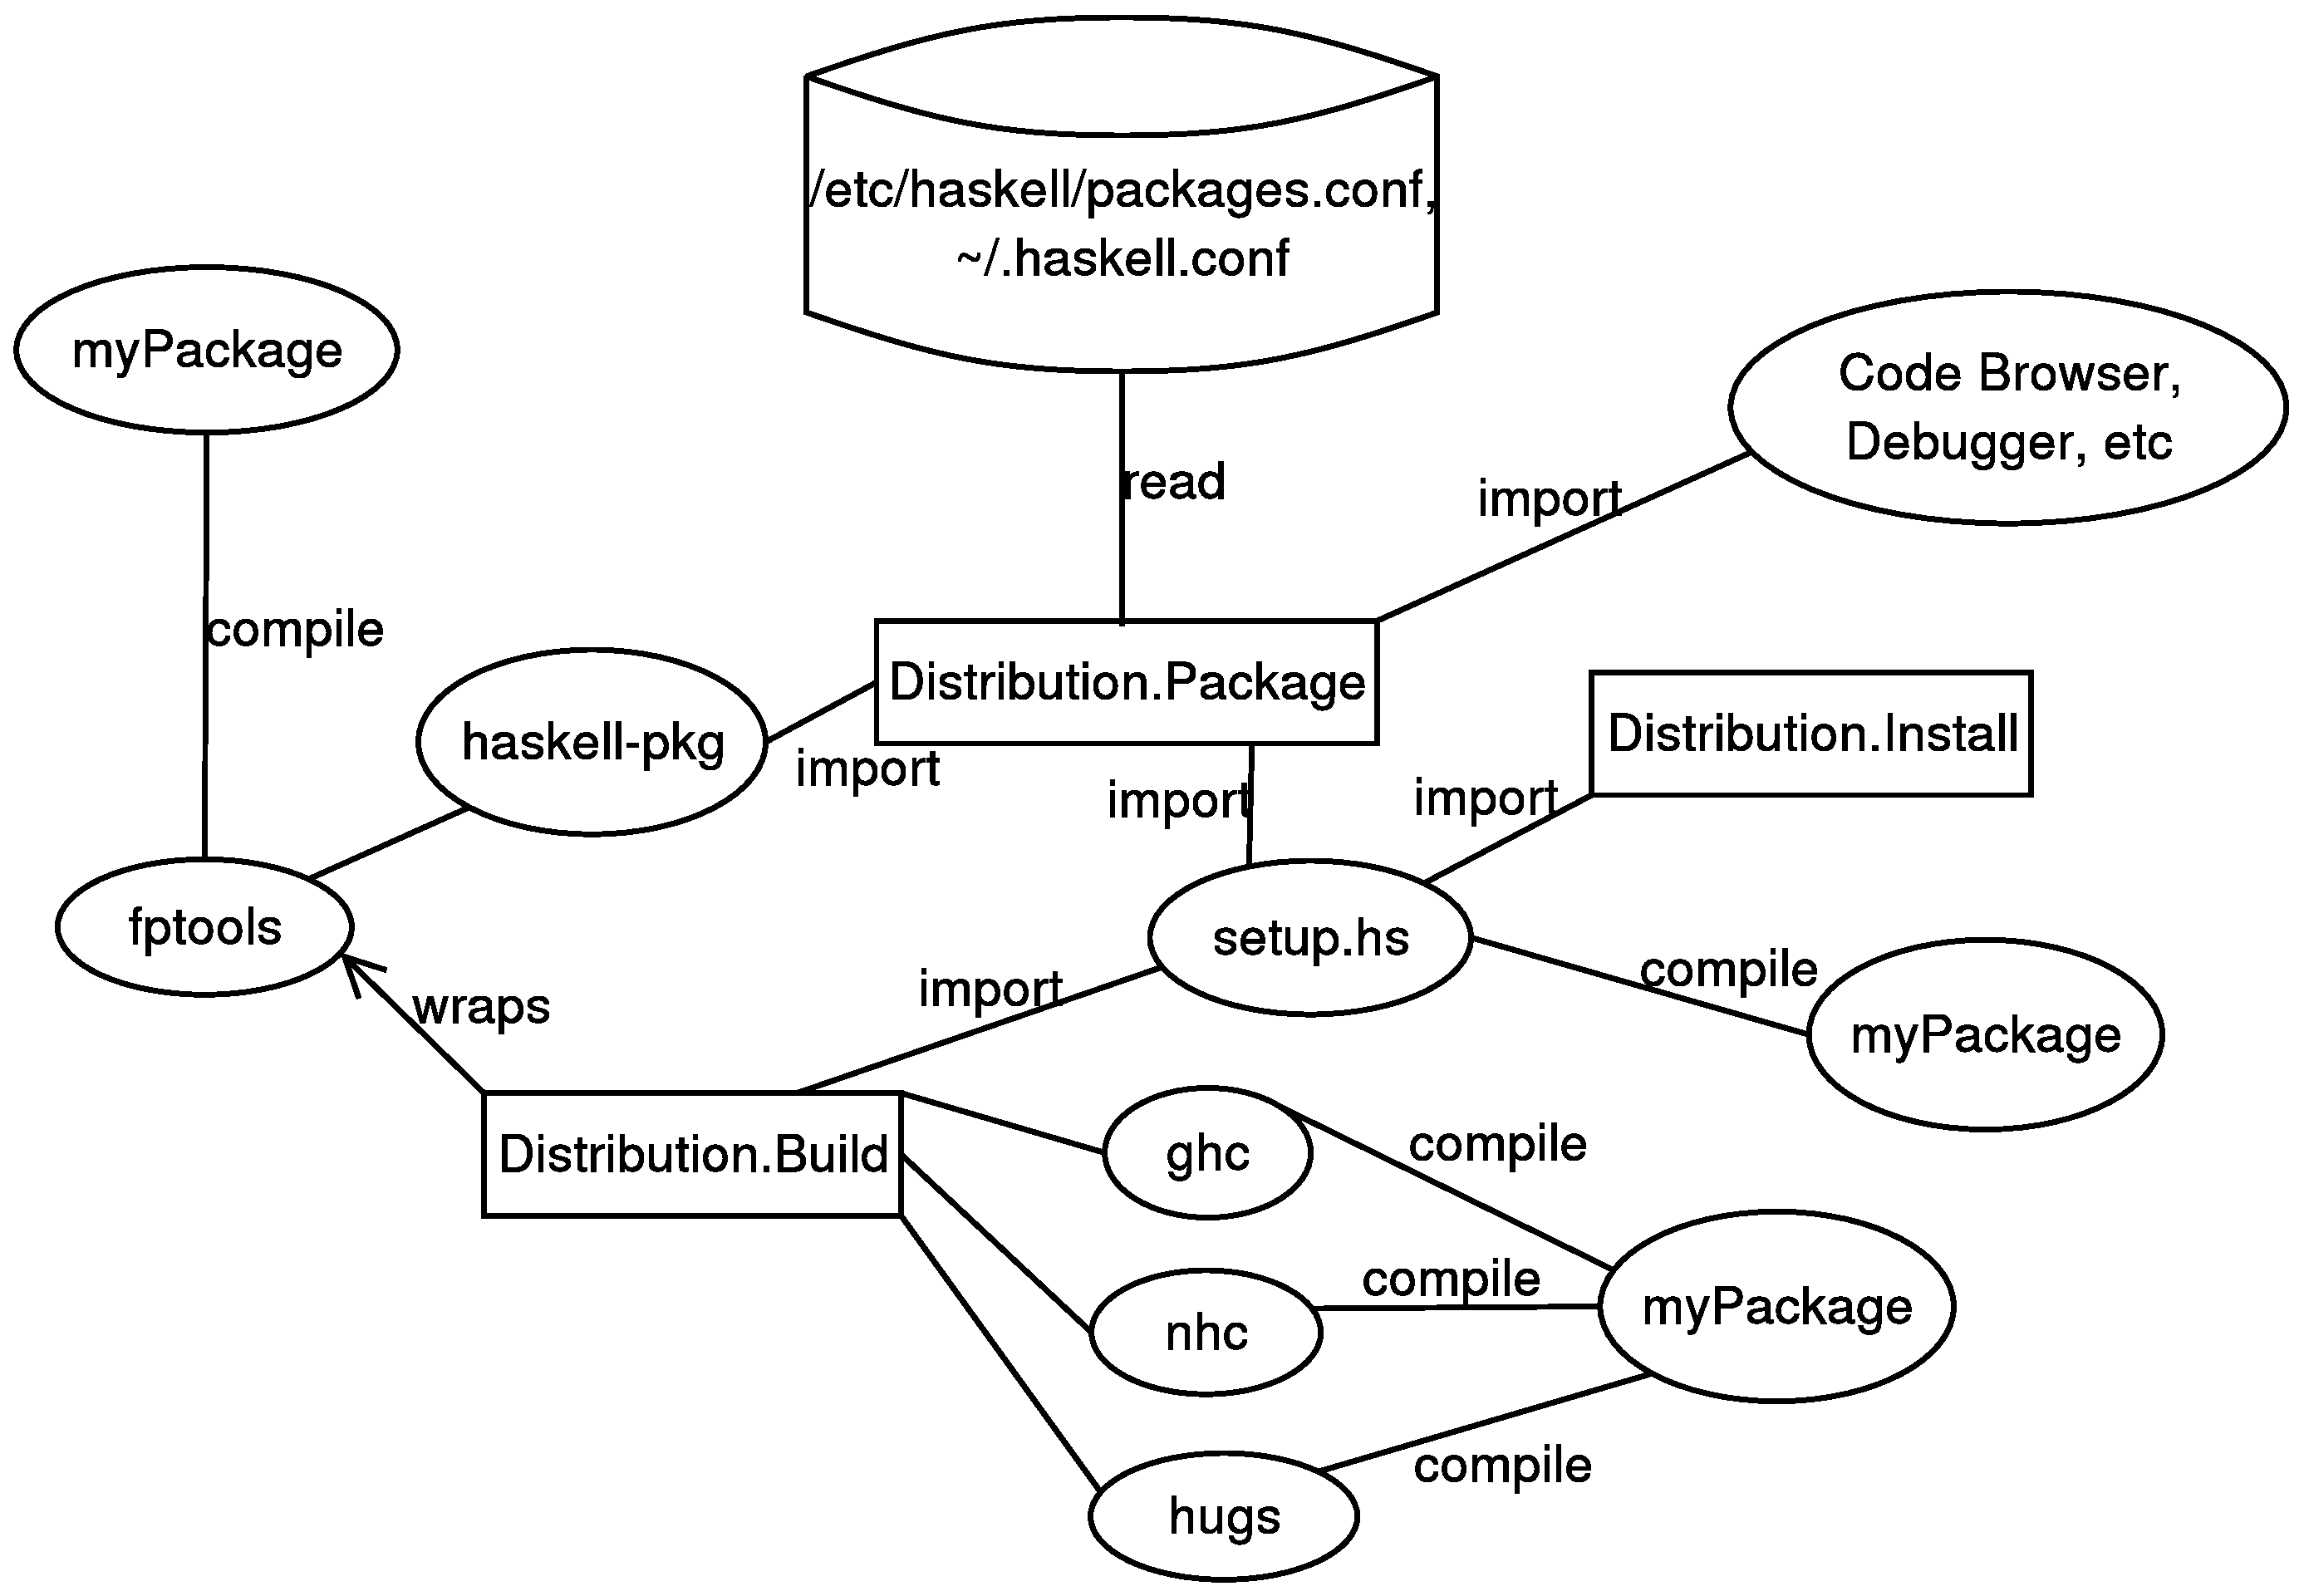
\includegraphics[width=.9\textwidth]{WholeSystem.eps}
\end{slide}

%% ------------------------------------------------------------
\begin{slide}{End of Overview}
That is the end of the overview. At this point, I hope you understand:	
\begin{itemize}
  \item The motivation for this project
  \item Some implementation ideas for this project
  \item Who would use it and how
\end{itemize}
\end{slide}

%% ------------------------------------------------------------
%% Building Section
%% ------------------------------------------------------------

%% ------------------------------------------------------------
\begin{slide}{Building}
Why building is hard:
\begin{itemize}
  \item Several very different Haskell implementations
  \item A variety of operating systems and hardware architectures
  \item Lots of preprocessors and foreign libraries
\end{itemize}
\end{slide}

%% ------------------------------------------------------------
\begin{slide}{Building: Basic strategy}
\begin{itemize}
  \item For simple tools like Haskell modules, leverage HMake's
  abilities and create a Haskell-based system (which may evolve to do
  more complex tasks.)

  \item Complex systems can use ``fptools'' or Yale's Make-based
  system, or their own build system.

  \item All systems will be wrapped in a common veneer (Haskell
  program) so they look the same to the average user, and to layered
  tools (like Debian).

\end{itemize}
\end{slide}

\begin{slide}{Tasks for Distribution.Build}
API For:
\begin{itemize}
  \item Compiling for a particular Implementation (like hmake)
  \item Compiling for all installed implementations
  \item Abstracting some implementation-specific flags
\end{itemize}
Can be used for:
\begin{itemize}
  \item Asking compilers to build Haskell code
  \item Dealing with some preprocessors
  \item Building higher-level tools on top (later slide)
  \item Recompiling when a new Implementation is installed
  \item Implementing a generic /usr/bin/haskell (like hi)
\end{itemize}
\end{slide}

%% ------------------------------------------------------------
%% Installation Section
%% ------------------------------------------------------------

%% ------------------------------------------------------------
\begin{slide}{Installation}
The main feature of the Installation Module is a script which imports
Distribution.Build, and interfaces with the packaging mechanisms
discussed below.
\end{slide}

%% ------------------------------------------------------------
\begin{slide}{Setup.hs Strategies}
\begin{itemize}
  \item \#!/usr/bin/env haskell (something haskell-interactive inspired?)
  \item Import Distribution.\{Build,Install,Package\} which can take care of major tasks
  \item main = distributionMain Package\{...insert package meta info here...\}
  \item Standard libraries may need richer OS operations
  \item ...but this is a good thing, it can help Haskell to get more market share in the scripting area
\end{itemize}
\end{slide}

%% ------------------------------------------------------------
\begin{slide}{Command-line arguments}
./Setup.hs
\begin{itemize}
  \item install-\{default,all,nhc,ghc,hugs\}
  \item build-\{default,all,nhc,ghc,hugs\}
  \item bdist-\{deb,rpm\}
  \item sdist --makes a tarball on unix
\end{itemize}
\end{slide}

%% ------------------------------------------------------------
\begin{slide}{Example Setup Program}
\begin{small}
\begin{verbatim}
#!/usr/bin/env haskell
import DistUtils.Core
import DistUtils.ToolInfo

toolInfo = (basicPackage (OtherTool "HUnit")
                         (Version 1 0 0))
	   {haskellSources=[
			    "HUnitLang98.lhs","HUnitLangExc.lhs",
			    "Terminal.lhs", "HUnitTest98.lhs", ...],
	    docs = ["Example.hs", "Guide.html", ...]}

main = distUtilsMain toolInfo
\end{verbatim}
\end{small}
\end{slide}

%% ------------------------------------------------------------
%% Packaging Section
%% ------------------------------------------------------------

%% ------------------------------------------------------------

% FIX: Disclaimer: saying I know that GHC, NHC, and Hugs already have their own (partial) solutions to this problem, but a grand-unified packaging systems gives us a lot :)..

\begin{slide}{Packaging}
  Much of this becomes easier with a more generic package system,
  which has benefits outside of this project.
\end{slide}

%% ------------------------------------------------------------
\begin{slide}{Jobs of a Packaging System}
  \begin{itemize}
  \item Track which Haskell Implementations are installed
  \item Track which preprocessors are installed
  \item Track which libraries and tools are installed
  \item Find the source code for modules when needed
  \end{itemize}
\end{slide}
%% ------------------------------------------------------------
\begin{slide}{Packaging}
   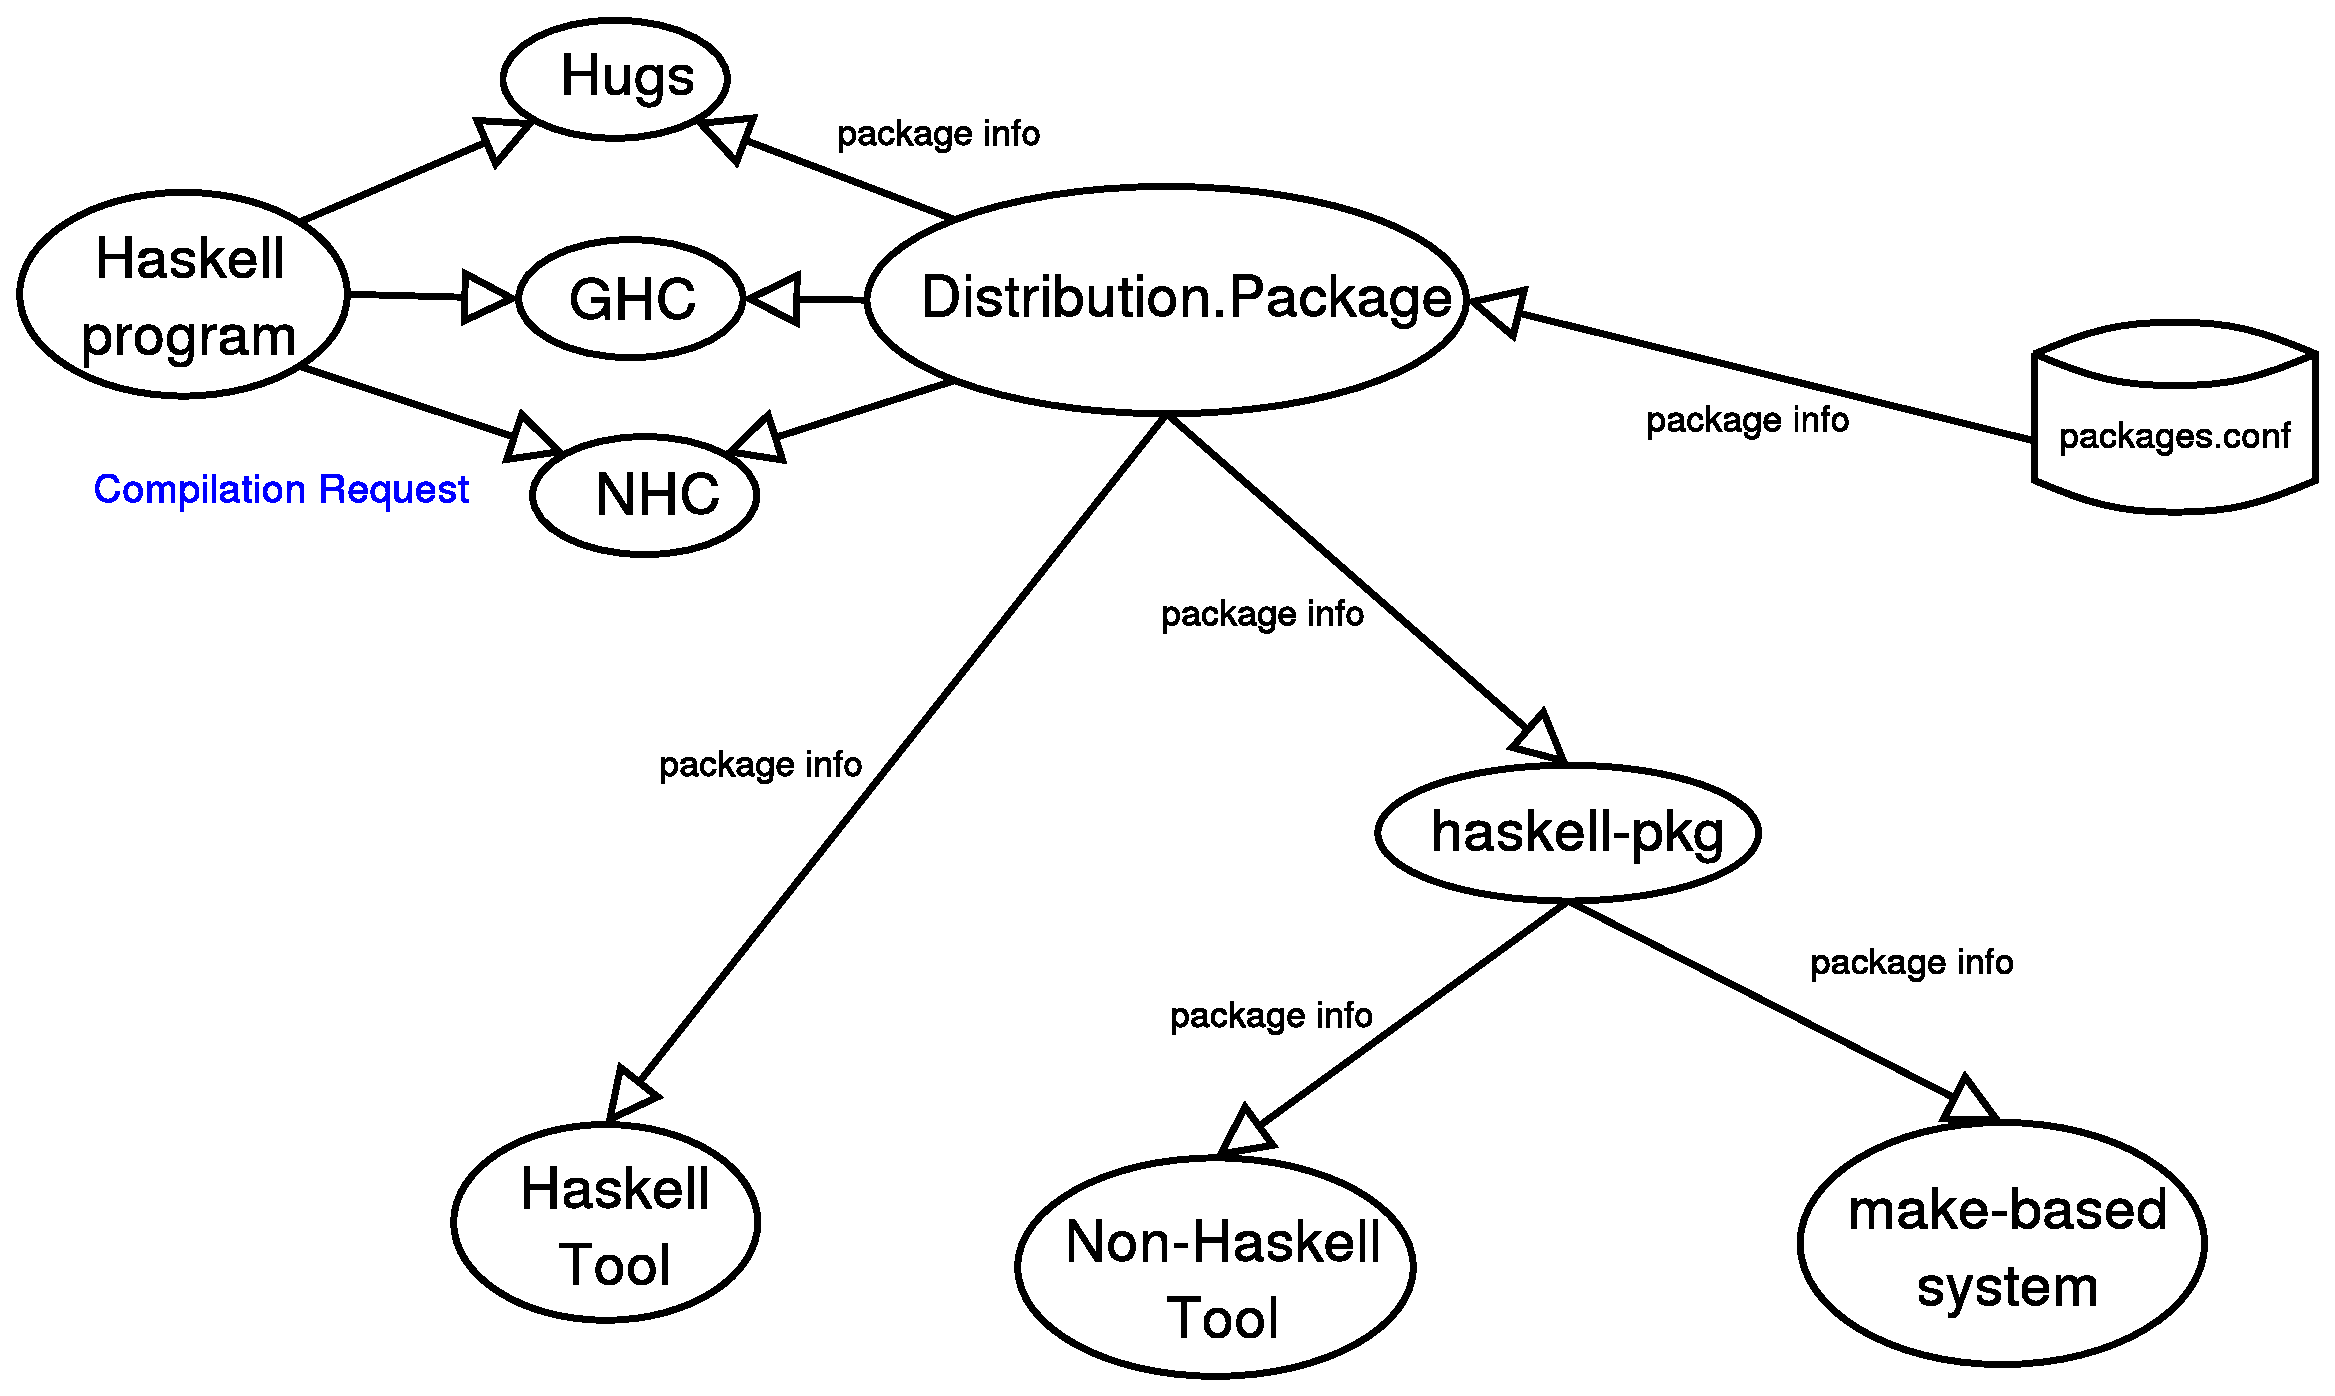
\includegraphics[width=.9\textwidth]{Packaging.eps}
\end{slide}

%% ------------------------------------------------------------
\begin{slide}{Package Meta Information}
Think of debian/control combined with Package.conf
\begin{itemize}
  \item \emph{Things the build system cares about:} Source Files, Build Flags, Build Dependencies
  \item \emph{Things the build system doesn't care about:} Name, Dependancies, Description, Version, License Information, Home Page
\end{itemize}
\end{slide}

%% ------------------------------------------------------------
\begin{slide}{System Overview}
   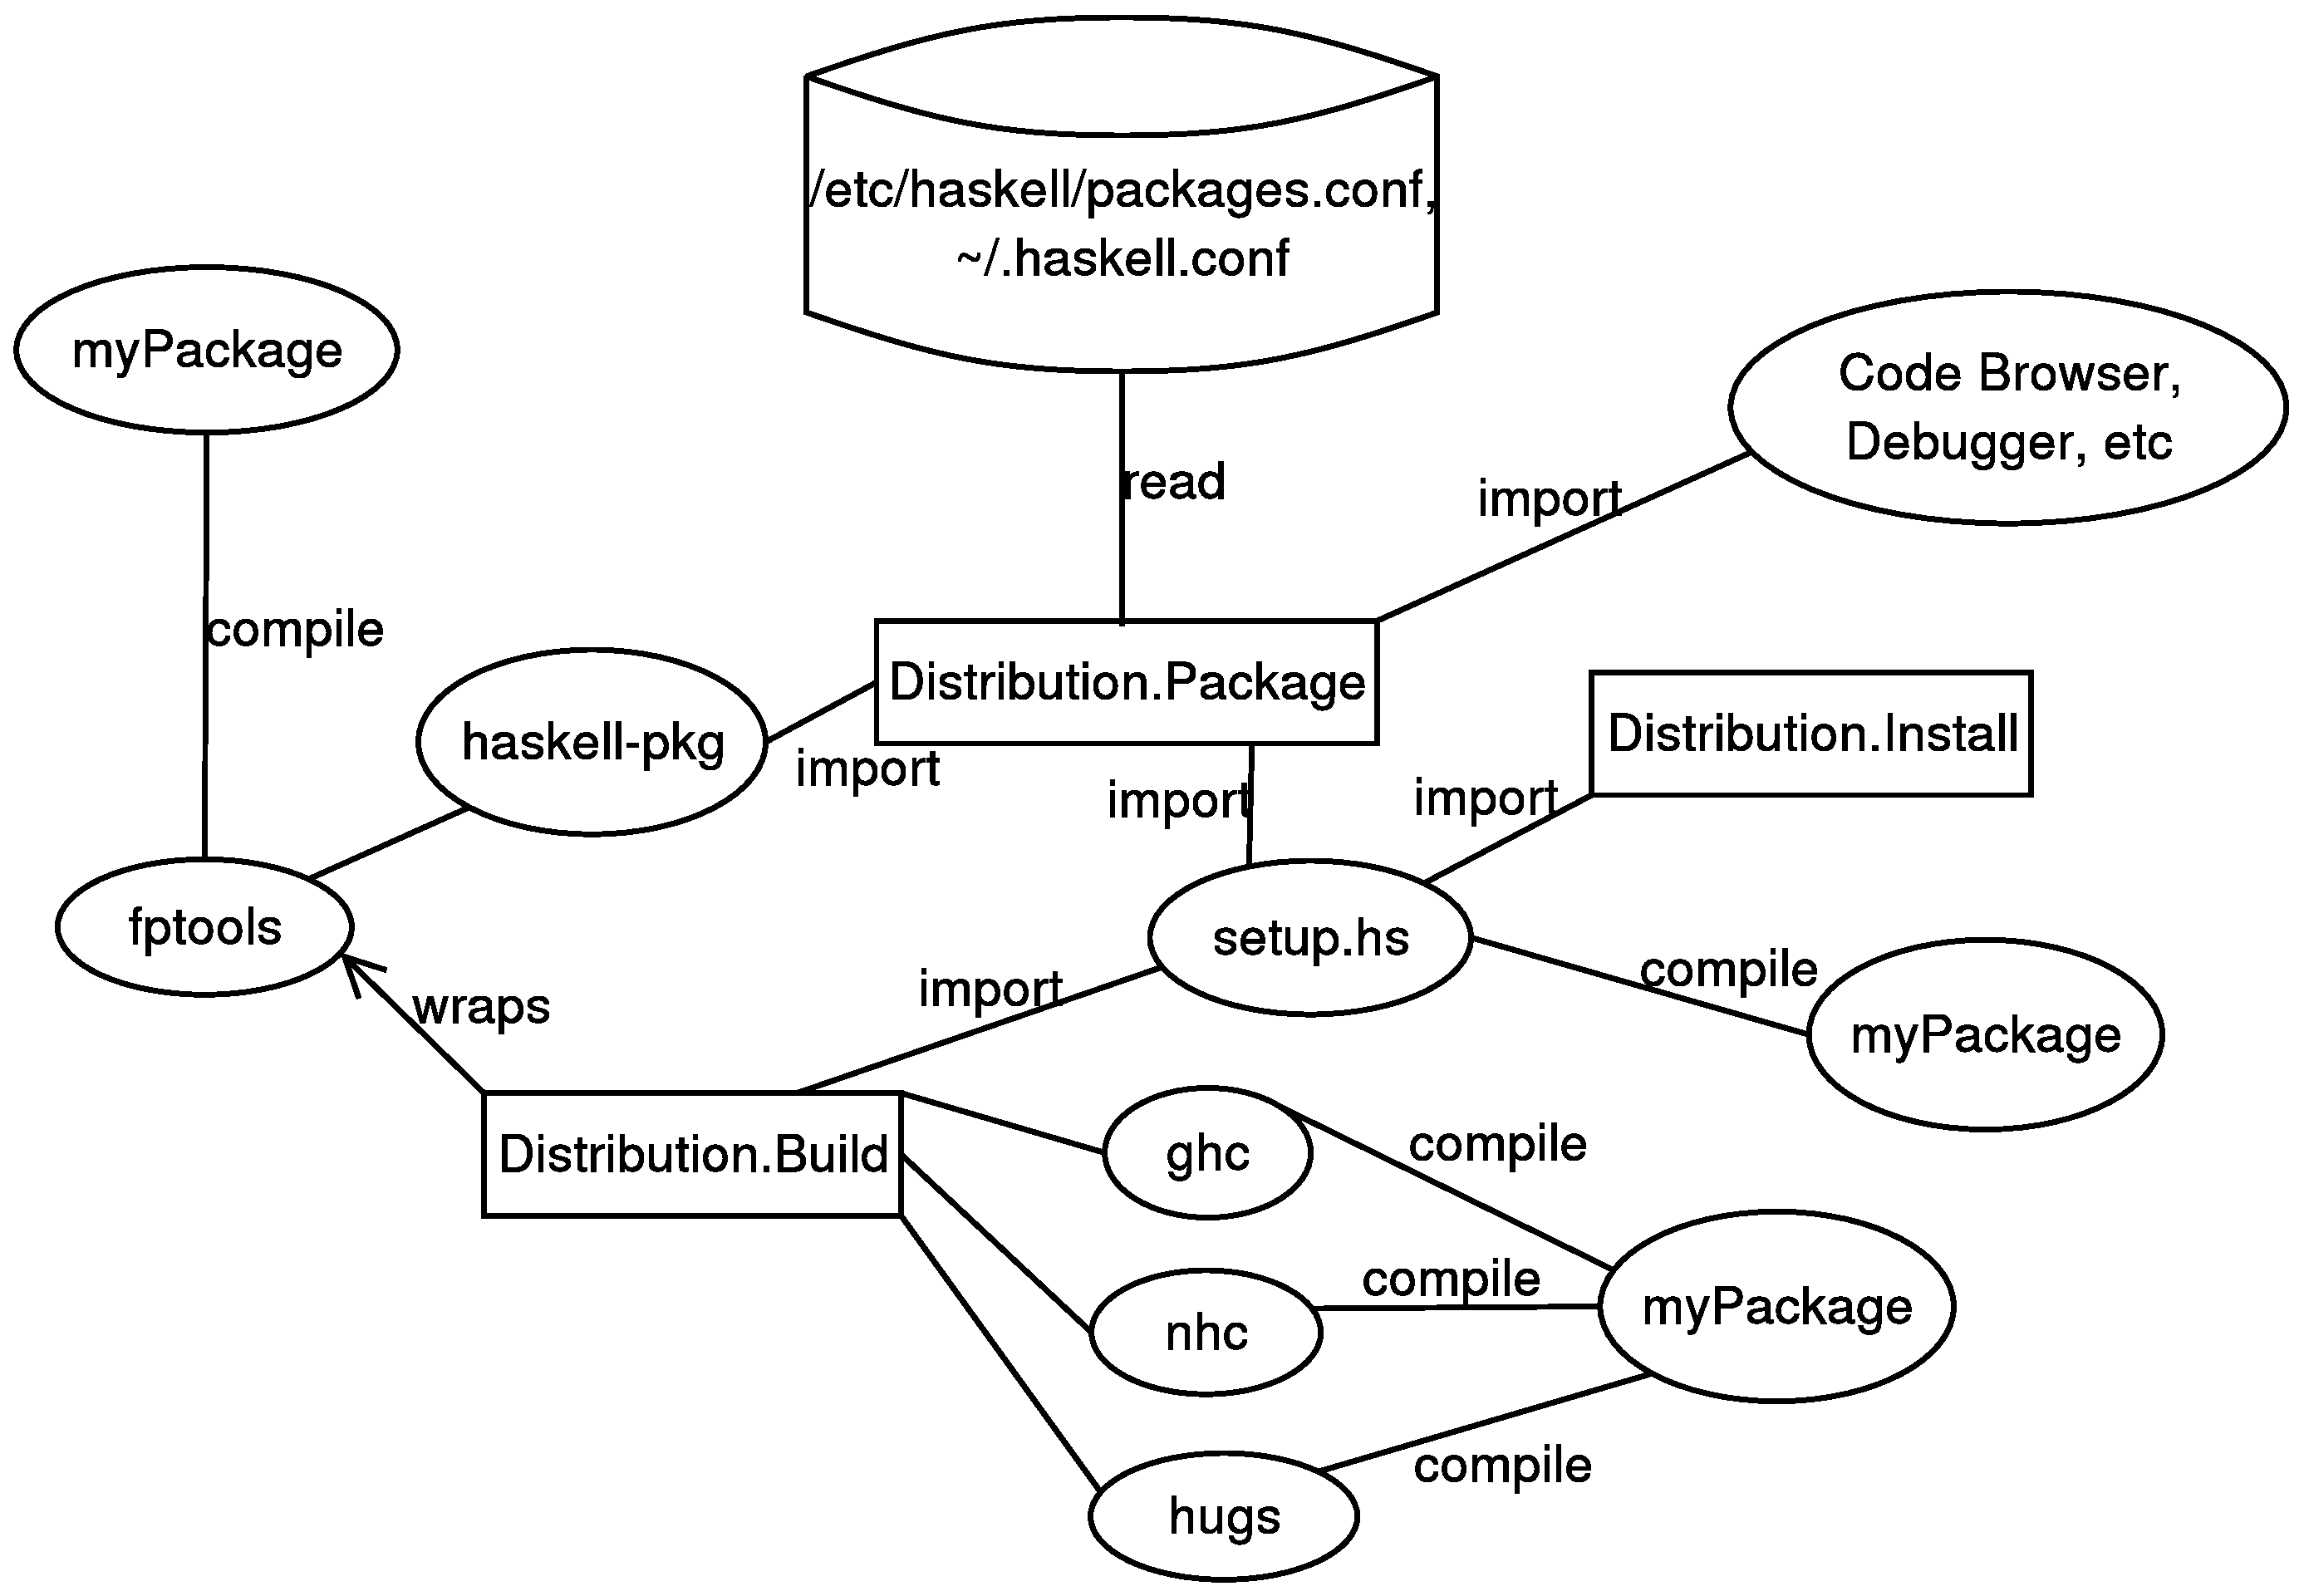
\includegraphics[width=.9\textwidth]{WholeSystem.eps}
\end{slide}



% SLIDE: side benefits ... (see tools support?)
% SLIDE: What would haskell implementers have to do to make the package system work
% - Haskell Implementation configure scripts would have to find packages.conf


%% ------------------------------------------------------------
%% Tool Support Section
%% ------------------------------------------------------------

\begin{slide}{Tools layered on Packaging System}
\begin{itemize}
  \item Build \& Install system
  \item Debuggers which need to instrument code
  \item Source code browsers
  \item The Glorious Glasgow Haskell Compiler Source Code Deleter (find other versions of software and ``repair'' any possible type errors)
\end{itemize}
\end{slide}

%% ------------------------------------------------------------
\begin{slide}{Layered Tools} % FIX: mentioned in a previous slide, remember
\begin{itemize}
  \item Creating distribution packages (Debian, FreeBSD, Windows, etc.)
  \item Web database of Haskell tools
  \item Installation (usually already there)
  \item Removal (often not there)
  \item Package registering and rebuilding
  \item Downloading and installing dependancies (job of parent system?)
  \item Verifying authenticity of packages (via cryptographic signature)
\end{itemize}
\end{slide}

%% ------------------------------------------------------------
\begin{slide}{Conclusions \& Directions}
  \begin{itemize}
  \item I have implemented a prototype (which interfaces with Debian's
  build system), but its blocked on a packaging system
  \item After HIM I will write a new proposal and try to create consensus
   \item But where do you think I should direct my attention (make-based system? CPAN-type archive? Distribution module?)
   \item My opinion: Packaging decisions, then Distribution module
  \end{itemize}
\end{slide}

%% ------------------------------------------------------------
\begin{slide}{Discussion}
(Assuming that we haven't run overtime and everyone is ready to go to lunch)
\end{slide}
% SLIDE: You may think its the job of the parent system, but some ``parent systems'' don't have packaging mechanisms, windows in particular, solaris maybe
% SLIDE: Does CPAN offer some of these same services?


%% ------------------------------------------------------------
%% Misc. Section
%% ------------------------------------------------------------

% Overview of everything thats being asked of implementation authors
% - include Distribution module
% - conform to the package interface
% - ...
% - ?
% - profit


%% ------------------------------------------------------------
%% Status Section
%% ------------------------------------------------------------

% - haskell experimental archive
% - distutils basic implementation
% - two make-based build systems
% - hmake
% - ...

\end{document}

% Decisions to make
- Packaging
- standard arguments to Setup.hs
- Name Where to focus efforts right now, review status in particular,
- what should I work on Should we encourage people to help out w/ the
- make-based systems?


%% Tools layered on haskel-dot-distribution (reuse)
- CPAN
- calculate dependancies between modules - could be used by haddock for instance
- Distribution.install - can be used to build an packaging system (like dpkg or rpm) in Haskell
- DARCS could use...
- bugtracker could use...
- tags / emacs / IDE could use...
- non-haskell programs which want to inter-operate w/ haskell programs could use --toolinfo
- debuggers need to know where packages go!(source code analysis for debugging and testing can often use a variety of information related to building)

%% what this doesn't solve...
- Packaging for Debian (a build system could do this with more meta-information)
-- distributing binaries is still a pain unless we can automate the packaging somewhat
- Tracking installed packages so the haskell implementations know where to find them (should be handled by the implementations)
- versioned dependancies
- installation of new haskell implementations

Notes: 
- Do we really want to duplicate debian / freeBSD, RPM, etc? aren't they duplicating eachother enough?!
- LIP Service to describe the suite of tools.  haskell-dot-distribution to describe the module


%%% Local Variables: 
%%% mode: latex
%%% TeX-master: t
%%% End: 

